\begin{figure}
  \centering
  \begin{subfigure}[t]{0.42\textwidth}
    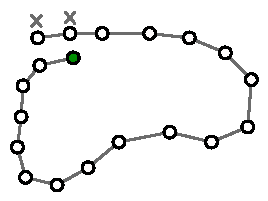
\includegraphics[width=\linewidth]{img/blob-overlap.pdf}
    \caption{A Blob with an initial overlap. To resolve, remove points
      at the end of the stroke marked with X's.}
    \label{fig:blob-overlap}
  \end{subfigure}
  \hspace{1cm} % spacing, do what you need
  \begin{subfigure}[t]{0.42\textwidth}
    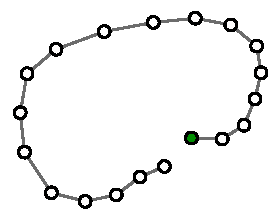
\includegraphics[width=\linewidth]{img/blob-gap.pdf}
    \caption{A Blob with an initial gap. No further action is needed.}
    \label{fig:blob-gap}
  \end{subfigure}
  \caption[Blobs: overlap vs. gap]{Two Blob shapes just before
    adjusting the start/end to match. The first is an overlap, the
    second is a gap. In case of an overlap, remove points from the end
    of the sequence until it becomes a gap. These define the initial
    spline control points.}
  \label{fig:blob}
\end{figure}
